\documentclass[conference]{IEEEtran}

\usepackage{iftex}
\ifXeTeX
  \usepackage{fontspec}
  \setmainfont{texgyretermes}[Extension=.otf,UprightFont=*-regular,BoldFont=*-bold,ItalicFont=*-italic,BoldItalicFont=*-bolditalic]
\fi

\usepackage{cite}
\usepackage{amsmath,amssymb}
\usepackage{graphicx}
\usepackage{booktabs,array}
\usepackage[section]{placeins}
\renewcommand{\topfraction}{0.85}
\renewcommand{\bottomfraction}{0.6}
\renewcommand{\textfraction}{0.12}
\renewcommand{\floatpagefraction}{0.8}
\setcounter{topnumber}{3}
\setcounter{bottomnumber}{2}
\setcounter{totalnumber}{4}
\usepackage[font=footnotesize,labelfont=bf,labelsep=colon,justification=justified,singlelinecheck=false]{caption}
\usepackage[font=footnotesize]{subfig}
\usepackage{url}
\usepackage[hidelinks,pdftitle={Can Ray-Tracing Hardware Accelerate SPH? Neighbourhood Search from CPU Threads to RT Cores},pdfauthor={Aditya Melinkeri, Ria Arora, Anirban Deshmukh, Prajakta Bandgar}]{hyperref}

\makeatletter
\renewcommand\thesection{\arabic{section}}
\renewcommand\thesubsection{\thesection.\arabic{subsection}}
\renewcommand\thesubsubsection{\thesubsection.\arabic{subsubsection}}
\renewcommand\thesectiondis{\thesection}
\renewcommand\thesubsectiondis{\thesubsection}
\renewcommand\thesubsubsectiondis{\thesubsubsection}
\renewcommand\thetable{\arabic{table}}
\renewcommand\section{\@startsection{section}{1}{\z@}%
  {2.2ex plus 1ex minus .4ex}{1.0ex plus .2ex}{\normalfont\large\bfseries}}
\renewcommand\subsection{\@startsection{subsection}{2}{\z@}%
  {1.6ex plus .6ex minus .3ex}{0.6ex plus .2ex}{\normalfont\normalsize\bfseries}}
\renewcommand\subsubsection{\@startsection{subsubsection}{3}{\z@}%
  {1.2ex plus .4ex minus .2ex}{0.4ex}{\normalfont\normalsize\bfseries\itshape}}
\renewenvironment{abstract}%
  {\noindent\small\textbf{Abstract}\hspace{0.6em}\itshape\ignorespaces}%
  {\par\vspace{0.8ex}\noindent\rule{\columnwidth}{0.4pt}\par\vspace{0.4ex}}
\makeatother
\captionsetup[figure]{name=Figure}
\captionsetup[table]{name=Table,position=top}

\begin{document}

\title{\bfseries Can Ray-Tracing Hardware Accelerate SPH?\\
Neighbourhood Search from CPU Threads to RT Cores}

\author{\IEEEauthorblockN{Aditya Melinkeri, Ria Arora, Anirban Deshmukh, Prajakta Bandgar}
\IEEEauthorblockA{November 2026}}

\maketitle

% ======================================================================
\begin{abstract}
Smoothed Particle Hydrodynamics (SPH) is a mesh-free method for simulating fluids, used in computer graphics, astrophysics and engineering. Most of its cost lies in neighbourhood search: in our sequential C++ solver, finding each particle's neighbours takes 93.6\% of a time step at 2,030 particles and 99.3\% at 30,016. We follow one solver from a sequential baseline through OpenMP multithreading, a uniform-grid (spatial hashing) search and a CUDA port, and finally replace the grid with a search built on the ray-tracing (RT) cores of recent NVIDIA GPUs, which earlier work has shown can accelerate fixed-radius neighbour queries. On a 24-core CPU the all-pairs solver reaches a 15.4$\times$ speed-up at 99,960 particles with an estimated serial fraction near 1\%, and the grid is a further 229$\times$ faster at the same thread count. On the GPU, the single-precision grid is 37--40$\times$ faster than the 24-thread CPU grid from $10^6$ particles upward. At SPH neighbour counts (about 80 per particle), however, RT-core search is 3--4$\times$ slower than a sort-based GPU grid on two GPU generations, for both density and force evaluation. We trace the published RT-core advantages to comparison conditions that SPH does not share, chiefly double-precision grid baselines, truncated searches and very sparse neighbourhoods.
\end{abstract}

% ======================================================================
\section{Introduction}

Smoothed Particle Hydrodynamics (SPH) represents a continuum as a set of particles that carry mass, velocity and other properties, and it evaluates every field by smoothing over nearby particles with a kernel function. It was introduced independently by Lucy~\cite{lucy1977} and by Gingold and Monaghan~\cite{gingold1977} in 1977 to study non-axisymmetric problems in stellar astrophysics, where a fixed mesh is a poor fit for matter that collapses, rotates and fragments. Astrophysics remains one of its main uses, from star formation and the giant impact thought to have formed the Moon~\cite{canup2001} to cosmological simulation~\cite{springel2010}. Because the particles move with the material, SPH also handles free surfaces, splashing and large deformations naturally, which has made it a standard tool in engineering for free-surface and coastal flows~\cite{crespo2015dualsphysics}. In computer graphics, M\"uller \emph{et al.}~\cite{muller2003particle} showed that SPH could produce interactive liquids, and it has since become a standard tool for visual effects and games~\cite{koschier2022survey}.

The usefulness of SPH has always been limited by its cost. Fine detail requires many particles, a stable explicit time step is short, and a single simulation may need millions of particles advanced over thousands of steps. Optimisation has therefore followed the hardware. Ihmsen \emph{et al.}~\cite{ihmsen2011parallel} showed how to parallelise an SPH solver efficiently on multi-core CPUs. Harada \emph{et al.}~\cite{harada2007sph} ran SPH on GPUs, first through graphics shaders. With CUDA came complete GPU solvers such as DualSPHysics~\cite{crespo2015dualsphysics}, which report order-of-magnitude speed-ups over CPU code. More recent work reduces precision where accuracy allows, using single-precision arithmetic with cell-relative coordinates~\cite{mao2024mixed}.

Across these platforms one step recurs as the bottleneck: \emph{neighbourhood search}. A particle interacts only with particles closer than the kernel's support radius, so every density and force evaluation must first find that set. Comparing every particle with every other costs $O(N^2)$ distance tests per step. Because the particles move, the neighbour sets change and must be found again at every step. Dom\'inguez \emph{et al.}~\cite{dominguez2011neighbour} identify building neighbour lists as one of the most time-consuming parts of an SPH step. Our own measurements agree: in a sequential all-pairs solver, the two neighbour searches take 93.6\% of a step at 2,030 particles and 99.3\% at 30,016 (Section~\ref{sec:cpu}). Any serious acceleration of SPH is, first of all, an acceleration of neighbour search.

The literature has followed two main strategies to avoid the all-pairs scan. The first is \emph{tree-based}. Hierarchical trees, introduced for gravitational $N$-body problems by Barnes and Hut~\cite{barnes1986}, group nearby particles so that a query can skip whole regions of space. Astrophysical codes such as GADGET-2~\cite{springel2005} use them for both gravity and SPH neighbours, because trees adapt to particles whose smoothing lengths vary by orders of magnitude. Queries cost $O(\log N)$ each, so a full step costs $O(N\log N)$. The second strategy is \emph{cell-based}. Space is divided into a uniform grid whose cell size equals the search radius, so a particle needs to examine only its own cell and the adjacent ones. The idea comes from cell lists in molecular dynamics~\cite{hockney1988}. In graphics, Teschner \emph{et al.}~\cite{teschner2003optimized} hashed grid cells into a fixed-size table so that unbounded domains need no dense grid. Green's NVIDIA report~\cite{green2010cuda} gave the form now standard on GPUs: compute each particle's cell index, sort particles by it, and record where each cell begins. With bounded cell occupancy this costs $O(N)$ per step. For SPH with a single smoothing length, the uniform grid is the usual choice.

In 2018 NVIDIA's Turing architecture added a new kind of hardware unit to its GPUs: the \emph{RT core}~\cite{nvidia2018turing}. RT cores exist to make real-time ray tracing possible. Given a ray and a tree of bounding boxes around the scene (a bounding volume hierarchy, BVH), they find which boxes the ray passes through, in fixed-function hardware and in parallel with the GPU's ordinary cores. Programmers reach them through NVIDIA's OptiX library. Soon after, researchers began to use this hardware for problems that are not rendering, starting with point location in tetrahedral meshes~\cite{wald2019rtx}. RTNN~\cite{zhu2022rtnn} built a general fixed-radius and $k$-nearest-neighbour library on RT cores and reported large speed-ups over existing GPU neighbour-search libraries, and Meneses \emph{et al.}~\cite{meneses2026rtnn} extended RT-core fixed-radius search with further optimisations and with particle sets whose search radii vary. The common trick is simple. Each particle is wrapped in a box the size of the search radius, and a very short ray is launched from each query point. The boxes the ray ``hits'' are the candidates, and the hardware finds them by walking the BVH.

These results suggest an obvious question for SPH. Its bottleneck is exactly a fixed-radius neighbour search, and RT cores are now present in every recent NVIDIA GPU, from laptops to workstations. Yet the published speed-ups were measured on stand-alone search benchmarks, often against baselines that differ from a well-tuned SPH grid. We propose to build RT-core neighbour search into a complete SPH solver and to test whether it holds up against the classical approaches that SPH already uses, on equal terms: the same particles, the same physics, the same precision and the same GPU. To do this we develop one solver through every stage of the usual optimisation path:
\begin{itemize}
\item a sequential all-pairs C++ baseline, profiled stage by stage;
\item OpenMP multithreading on a 24-core CPU, with an analysis of what limits its scaling;
\item a uniform-grid (spatial hashing) search on the CPU and in CUDA;
\item an RT-core search through OptiX, compared with the GPU grid at SPH-like neighbour counts.
\end{itemize}
Section~\ref{sec:sph} summarises the SPH formulation, and Section~\ref{sec:valid} describes how the sequential solver was validated. Section~\ref{sec:cpu} presents the CPU parallelisation and the evidence that neighbour search dominates. Section~\ref{sec:search} describes the grid and BVH search structures, and Section~\ref{sec:rt} explains how RT cores are used for neighbour search.
Section~\ref{sec:gpuresults} presents the GPU benchmark protocol and results, including a controlled comparison of RT-core search with a CUDA grid. Section~\ref{sec:conclusion} summarises the findings and their limits.

% ======================================================================
\section{Smoothed Particle Hydrodynamics}\label{sec:sph}

\subsection{Kernel Interpolation}

SPH starts from an exact identity: any field $A$ can be written as an integral of itself against the Dirac delta,
\begin{equation}
A(\mathbf{r}) = \int A(\mathbf{r}')\,\delta(\mathbf{r}-\mathbf{r}')\,d\mathbf{r}'.
\end{equation}
The delta is replaced by a smooth \emph{kernel} $W$ of width $h$, the smoothing length (Fig.~\ref{fig:kernel}):
\begin{equation}
A(\mathbf{r}) \approx \int A(\mathbf{r}')\,W(\mathbf{r}-\mathbf{r}',h)\,d\mathbf{r}'.
\label{eq:integral}
\end{equation}
The kernel integrates to one, approaches the delta as $h\to0$, and, for the kernels used in practice, is exactly zero beyond a finite \emph{support radius} $R$. That last property is what makes neighbourhood search possible: only particles closer than $R$ contribute anything.

\begin{figure}[!htb]
\centering
\subfloat[Ideal Dirac delta]{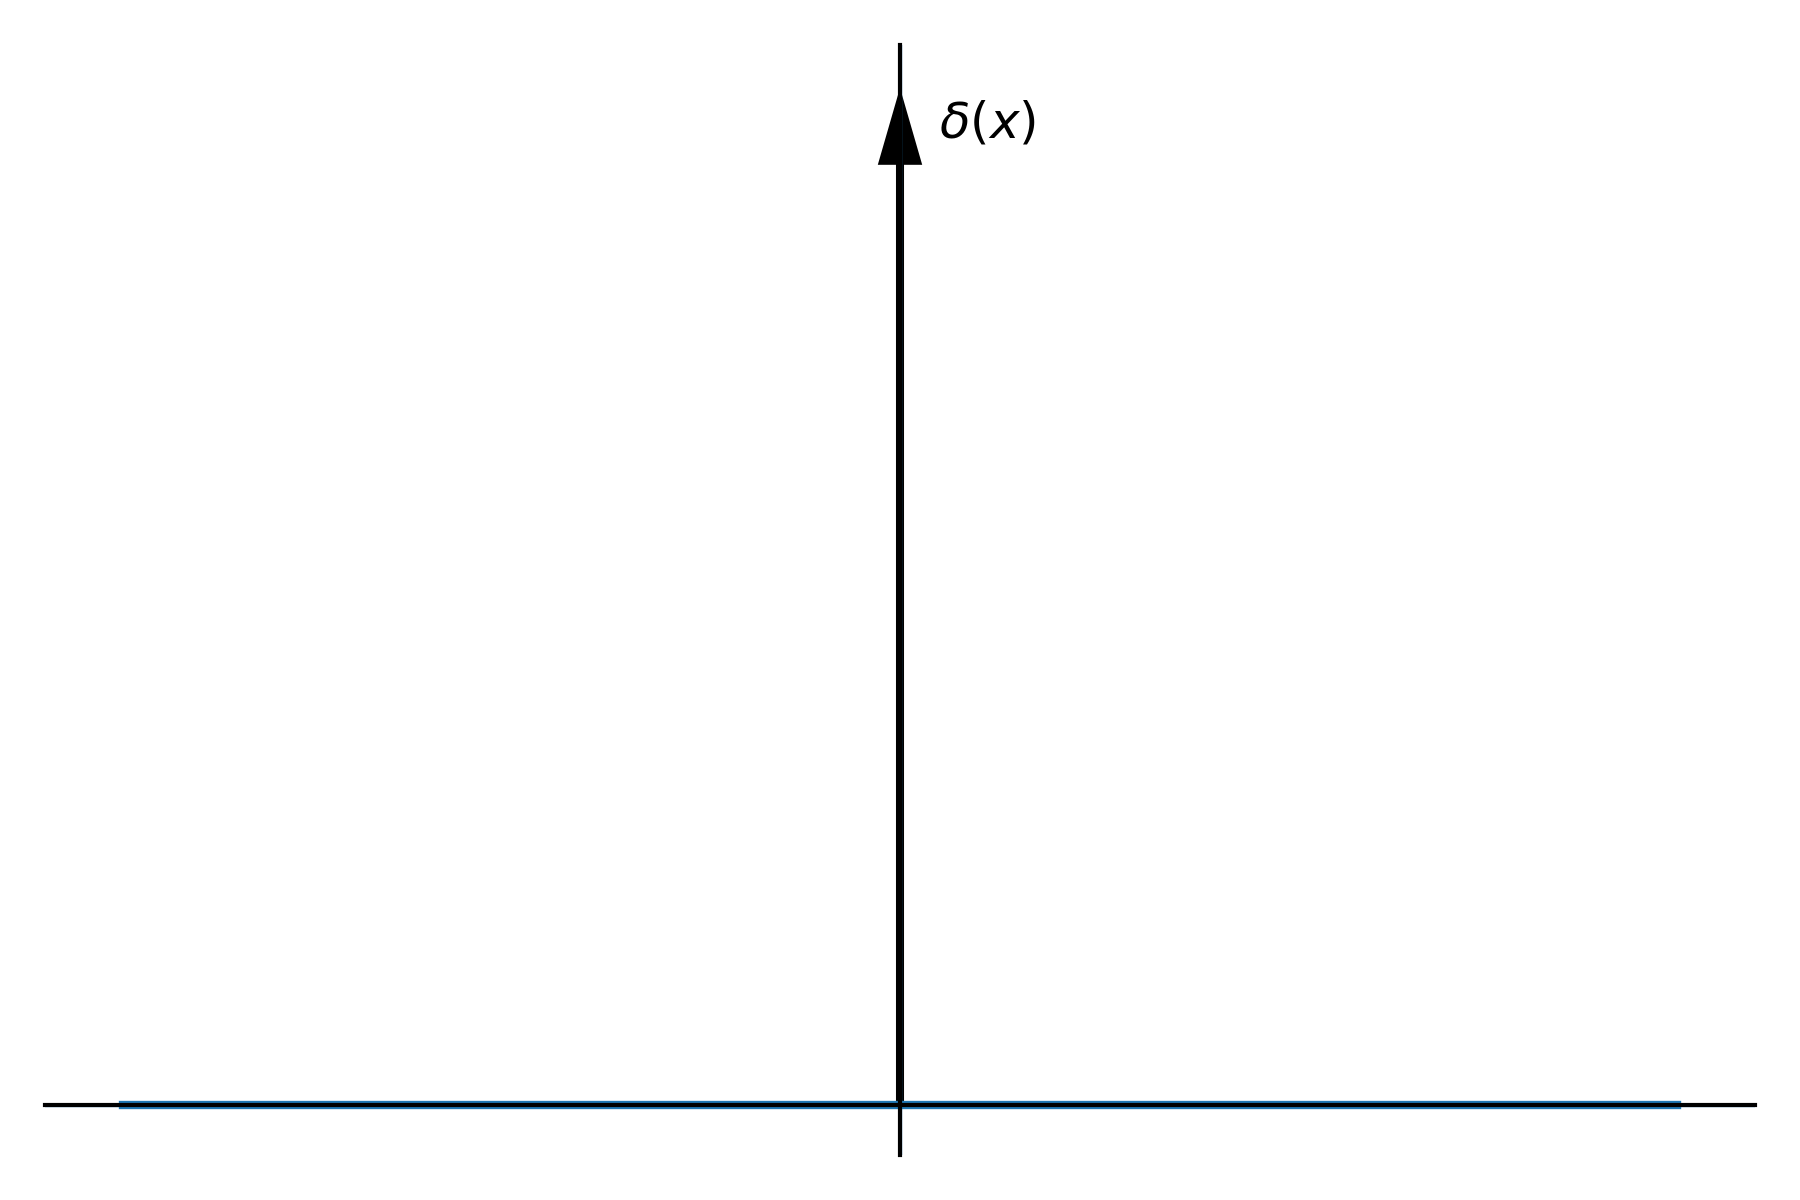
\includegraphics[width=0.47\columnwidth]{figures/dirac_true.png}}
\hfill
\subfloat[Kernel approximation]{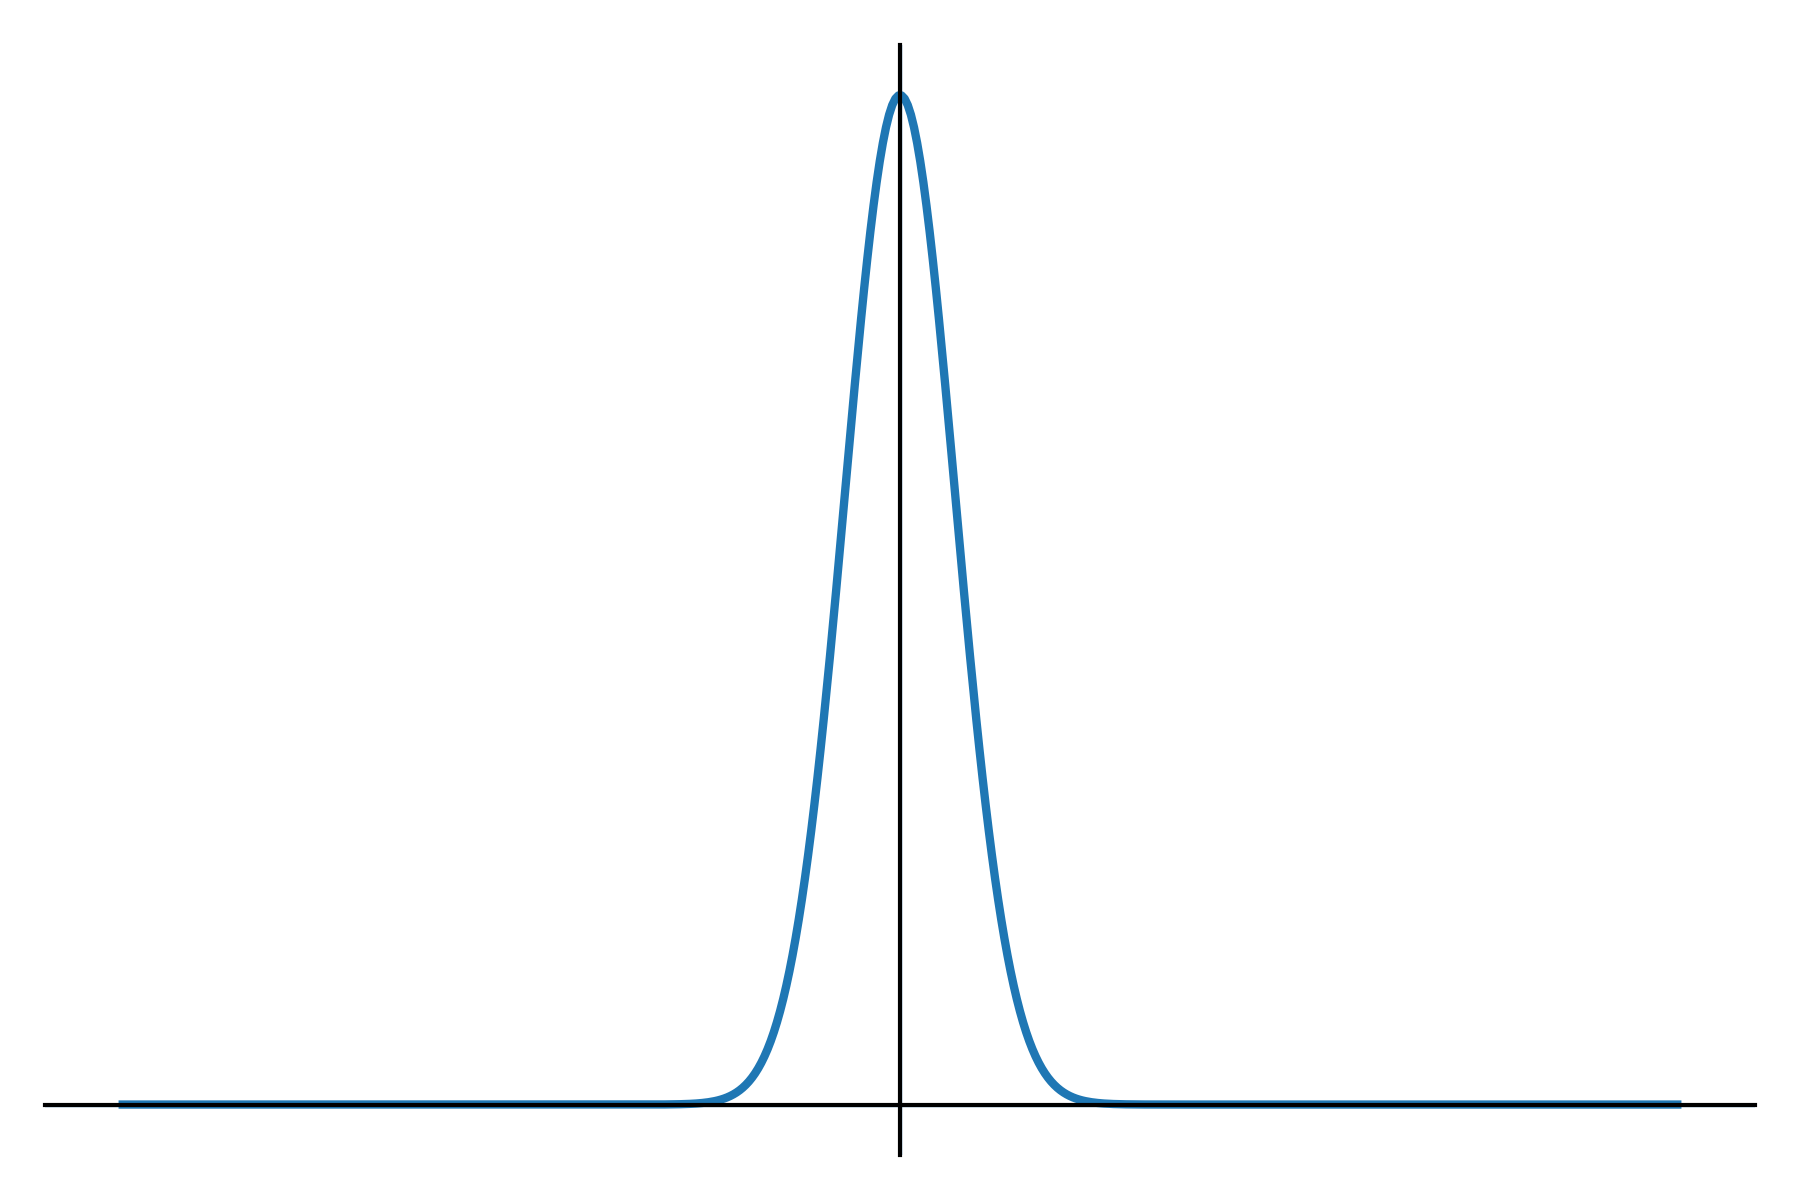
\includegraphics[width=0.47\columnwidth]{figures/gaussian.png}}
\caption{The Dirac delta and its approximation by a smoothing kernel. The kernel spreads the contribution of a point over a finite neighbourhood and falls to zero beyond the support radius $R$.}
\label{fig:kernel}
\end{figure}

\subsection{Particle Approximation}

The fluid is now divided into particles. Particle $j$ has mass $m_j$ and density $\rho_j$, so it represents a volume $m_j/\rho_j$. Replacing the integral in~\eqref{eq:integral} with a sum over particles gives
\begin{equation}
A_i = \sum_j \frac{m_j}{\rho_j}\,A_j\,W(r_{ij},h), \qquad r_{ij}=\lVert\mathbf{x}_i-\mathbf{x}_j\rVert .
\label{eq:sum}
\end{equation}
Substituting $A=\rho$ gives the density directly from the particle positions:
\begin{equation}
\rho_i = \sum_{j\in\mathcal{N}(i)} m_j\,W(r_{ij},h),
\label{eq:density}
\end{equation}
where $\mathcal{N}(i)=\{\,j : r_{ij}<R\,\}$ is the \emph{neighbour set} of particle $i$, including $i$ itself. Gradients follow the same pattern. Only the kernel depends on $\mathbf{x}_i$, so
\begin{equation}
\nabla A_i \approx \sum_{j\in\mathcal{N}(i)} \frac{m_j}{\rho_j}\,A_j\,\nabla_i W(r_{ij},h).
\label{eq:gradient}
\end{equation}
Spatial derivatives therefore become sums over neighbours of a kernel gradient that is known analytically. No mesh is needed.

\subsection{Governing Equations}

The fluid obeys the Navier--Stokes momentum equation,
\begin{equation}
\frac{D\mathbf{v}}{Dt} = -\frac{1}{\rho}\nabla p + \nu\nabla^2\mathbf{v} + \mathbf{g}.
\end{equation}
Because each particle moves with the fluid, the material derivative $D\mathbf{v}/Dt$ is simply the particle's acceleration, and the advection term of a mesh-based solver disappears.

Applying~\eqref{eq:gradient} directly to the pressure gives a force that is not symmetric between $i$ and $j$, so Newton's third law is violated and momentum is not conserved. M\"uller \emph{et al.}~\cite{muller2003particle} fix this by averaging the two pressures. Our solver uses the symmetric form of Monaghan~\cite{monaghan1992}:
\begin{equation}
\left(\frac{\nabla p}{\rho}\right)_i \approx \sum_{j\in\mathcal{N}(i)} m_j\left(\frac{p_i}{\rho_i^2}+\frac{p_j}{\rho_j^2}\right)\nabla_i W(r_{ij},h).
\end{equation}
Pressure comes from density through a weakly compressible equation of state,
\begin{equation}
p_i = K(\rho_i-\rho_0),
\label{eq:eos}
\end{equation}
where $\rho_0$ is the target density and $K$ is a pressure multiplier, giving a reference sound speed $c_0=\sqrt{K}$. A particle denser than $\rho_0$ pushes its neighbours away, and a sparser one pulls them in.

Combining pressure, viscosity and gravity, the acceleration of a particle is
\begin{equation}
\mathbf{a}_i = -\sum_{j\in\mathcal{N}(i),\,j\ne i} m_j\left(\frac{p_i}{\rho_i^2}+\frac{p_j}{\rho_j^2}+\Pi_{ij}\right)\nabla_i W(r_{ij},h) + \mathbf{g},
\label{eq:accel}
\end{equation}
where
\begin{itemize}
\item $\mathbf{a}_i$ is the acceleration of particle $i$, and the sum runs over its neighbours $j$, excluding $i$ itself;
\item $m_j$ is the mass of neighbour $j$;
\item $p_i, p_j$ and $\rho_i, \rho_j$ are the pressures and densities of the two particles. The pressure term pushes a compressed pair apart, and because it is symmetric in $i$ and $j$, the two particles receive equal and opposite forces;
\item $\Pi_{ij}$ is Monaghan's artificial viscosity~\cite{monaghan1992}, a damping term that is non-zero only when $i$ and $j$ are moving towards each other and grows with their closing speed. It smooths the flow and removes spurious oscillations;
\item $\nabla_i W(r_{ij},h)$ is the kernel gradient, which points along the line joining the two particles, $\mathbf{x}_{ij}=\mathbf{x}_i-\mathbf{x}_j$, and sets how strongly each neighbour contributes;
\item $\mathbf{g}$ is gravitational acceleration.
\end{itemize}

\subsection{Choice of Kernel}

M\"uller \emph{et al.}~\cite{muller2003particle} use the Poly6 kernel for density and the Spiky kernel for pressure, and our first Python prototype followed them. The C++, CUDA and RT-core solvers in this paper use the cubic B-spline kernel~\cite{monaghan1985}, with $q=r/h$:
\begin{equation}
W(q,h)=\sigma_d
\begin{cases}
1-\tfrac{3}{2}q^2+\tfrac{3}{4}q^3, & 0\le q<1,\\[2pt]
\tfrac{1}{4}(2-q)^3, & 1\le q<2,\\[2pt]
0, & q\ge 2,
\end{cases}
\end{equation}
where $\sigma_2=10/(7\pi h^2)$ in two dimensions and $\sigma_3=1/(\pi h^3)$ in three. Its gradient is
\begin{equation}
\nabla_i W = \frac{\sigma_d}{h}\,\frac{\mathbf{x}_{ij}}{r_{ij}}
\begin{cases}
-3q+\tfrac{9}{4}q^2, & 0\le q<1,\\[2pt]
-\tfrac{3}{4}(2-q)^2, & 1\le q<2,\\[2pt]
0, & q\ge 2.
\end{cases}
\end{equation}
The kernel vanishes at $q=2$, so the support radius is $R=2h$. This radius sets the cell size of the grid in Section~\ref{sec:search} and the box size of the RT-core search in Section~\ref{sec:rt}.

\begin{figure}[!htb]
\centering
\includegraphics[page=5,width=0.7\columnwidth,keepaspectratio]{figures/report_figure_assets.pdf}
\caption{Finite-support interactions. Only particles inside the support circle of radius $R=2h$ contribute to the target particle; finding them is the neighbourhood search.}
\label{fig:support}
\end{figure}

\subsection{Simulation Loop}

Each time step advances all particles with a kick--drift--kick (leapfrog) integrator:
\begin{enumerate}
\item Choose $\Delta t$ from acoustic and force stability limits.
\item Half kick: $\mathbf{v}_i \leftarrow \mathbf{v}_i + \tfrac{1}{2}\Delta t\,\mathbf{a}_i$.
\item Drift: $\mathbf{x}_i \leftarrow \mathbf{x}_i + \Delta t\,\mathbf{v}_i$, then apply the wall boundaries.
\item \textbf{Find $\mathcal{N}(i)$} and compute densities with~\eqref{eq:density}.
\item Compute pressures with~\eqref{eq:eos}.
\item \textbf{Find $\mathcal{N}(i)$} and compute accelerations with~\eqref{eq:accel}.
\item Half kick: $\mathbf{v}_i \leftarrow \mathbf{v}_i + \tfrac{1}{2}\Delta t\,\mathbf{a}_i$.
\end{enumerate}
Steps 4 and 6 are the only steps that need the neighbour set, and both repeat it every step because the particles have moved. Every other step costs $O(N)$ and is trivially parallel. The rest of this paper is about making steps 4 and 6 cheap.

% ======================================================================
\section{Validating the Sequential Solver}\label{sec:valid}

Every faster solver in this paper is checked against the sequential C++ solver, so before optimising anything we made sure that this reference solver behaves physically. We wrote a small validation harness in Python that is independent of the solver. It generates the initial particles for a test scene, the solver runs the scene and writes out its particle states, and the harness then checks that output. Because the harness only reads output files, the same checks apply unchanged to the OpenMP and CUDA versions. Every scene gets three kinds of check: structural checks (no particle lost, no invalid values, no particle outside the tank), time-step checks (each step stays within the acoustic and force stability limits), and physics checks specific to the scene. The three scenes are listed in Table~\ref{tab:scenes}. All are two-dimensional, with a particle spacing of about 0.02~m and a rest density of 1000~kg/m$^3$.

\begin{table}[!htb]
\centering
\caption{Validation scenes.}
\label{tab:scenes}
\footnotesize
\begin{tabular}{@{}l r >{\raggedright\arraybackslash}p{1.35in} >{\raggedright\arraybackslash}p{0.8in}@{}}
\toprule
Scene & $N$ & Set-up & Tests \\
\midrule
Dam break & 98 & $0.146\times0.292$~m column in a 0.584~m square tank, 0.8~s & Collapse and front motion \\
Hydrostatic & 375 & 0.3~m of still water in a $0.5\times0.6$~m tank, 2~s & Rest state, pressure vs.\ depth \\
Momentum & 125 & Two unequal blobs collide, no gravity or walls, 0.6~s & Momentum conservation \\
\bottomrule
\end{tabular}
\end{table}

\subsection{Dam Break}

The dam break is the standard test for free-surface SPH~\cite{monaghan1994}. A column of water held against the left wall is released at $t=0$ and collapses under gravity. Martin and Moyce~\cite{martin1952} and Koshizuka and Oka~\cite{koshizuka1996} measured experimentally how fast the front of the water travels along the floor. Fig.~\ref{fig:dambreak} shows our run. The column collapses and spreads along the floor, and the front reaches the far wall after 0.23~s. The water then runs up that wall, falls back, and settles into a shallow layer by the end of the run. The front advances monotonically until it reaches the far wall, and the water at the left wall drops from the full 0.292~m column height until none remains there at 0.215~s. These are the expected features of a dam break.

\begin{figure}[!htb]
\centering
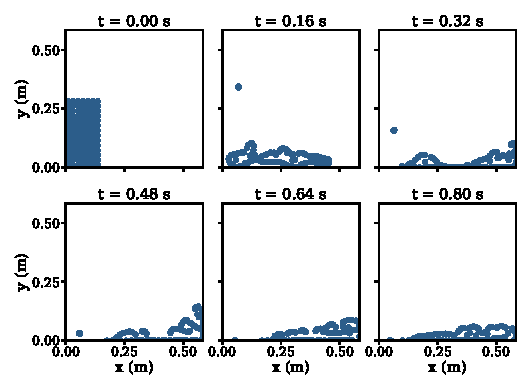
\includegraphics[width=\columnwidth,keepaspectratio]{figures/dambreak_snapshots.pdf}
\caption{Dam-break snapshots from the sequential solver. The column released at $t=0$ collapses, reaches the far wall at about 0.23~s, runs up it, and settles into a shallow layer.}
\label{fig:dambreak}
\end{figure}

Fig.~\ref{fig:energy} shows the mechanical energy of the run. With no energy entering the system, kinetic plus potential energy should only fall as viscosity dissipates it. From the first output frame onwards it does, decaying smoothly from 706 to 10.1 (in the solver's areal units). In that first frame, however, at $t=0.005$~s, the energy jumps from 61 to 706. The cause is the initial condition. The particles start on a regular lattice, so particles at the free surface and in the corners have fewer neighbours than interior particles, and their density sums come out too low. The corner particle, for example, starts at 530~kg/m$^3$ instead of 1000. The equation of state turns this deficit into large unbalanced pressure forces, which kick the particles in the first few steps. This cold-start transient is a known SPH artefact. It can be removed by relaxing the lattice before the run starts, which we have not done. As a result, the harness's energy check, which allows energy to rise at most 2\% above its starting value, fails on this transient.

\begin{figure}[!htb]
\centering
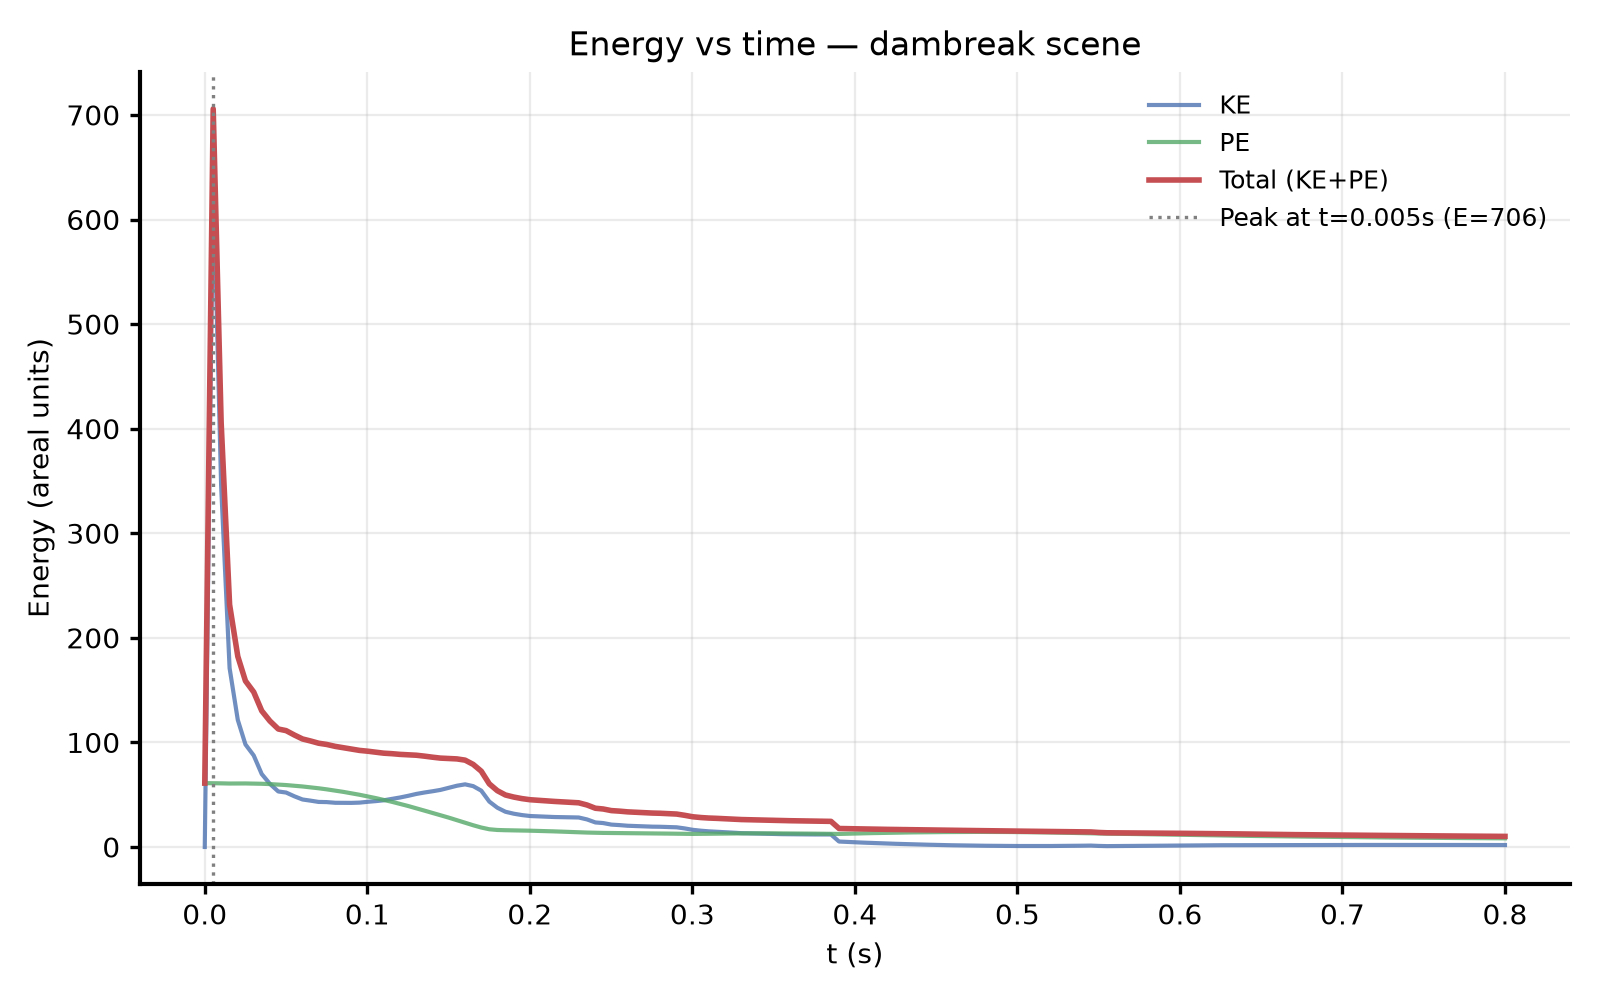
\includegraphics[width=\columnwidth,keepaspectratio]{figures/energy_vs_time_dambreak.png}
\caption{Kinetic, potential and total energy in the dam break. After a spike in the first frame, caused by the initial lattice, the total energy decays smoothly as viscosity dissipates it.}
\label{fig:energy}
\end{figure}

The dam-break result is qualitative. The harness can compare the front position against a digitised experimental curve, but we have not yet digitised one, so no quantitative comparison with experiment has been made. With only 98 particles the run is also coarse, and the measured front position is noisy in the first few frames.

\subsection{Hydrostatic Tank and Momentum Conservation}

Two simpler scenes test specific properties of the solver. In the \emph{hydrostatic} scene, a tank of still water should stay still. The run does settle: kinetic energy falls from a peak of 173.7 during the initial settling to $6.9\times10^{-4}$, and the interior density stays within 0.09\% of the rest density. Two discrepancies remain. The free surface settles 21\% lower than the nominal fill height. The pressure also rises with depth at only 0.30 of the expected rate $\rho_0 g$ (Fig.~\ref{fig:valid}(b)). We believe the wall model is responsible: walls are handled by clamping particles to the tank and reflecting their velocity, so the floor, rather than the fluid's pressure, carries part of the column's weight. We have not confirmed this. A ghost-particle wall that would test it was started but not completed.

In the \emph{momentum} scene, two blobs of fluid collide with gravity switched off and well away from the walls. Nothing outside the fluid acts on it, so its total momentum must stay exactly constant. This holds only if every force particle $j$ exerts on particle $i$ is matched by an equal and opposite force on $j$, which is what the symmetric form of~\eqref{eq:accel} guarantees. The largest relative drift over the run is $2.4\times10^{-16}$ (Fig.~\ref{fig:valid}(a)), at the level of double-precision rounding. This is the strongest of the three results, because it confirms that the force calculation, which every later solver reuses, is implemented correctly.

\begin{figure}[!htb]
\centering
\subfloat[Relative momentum drift, momentum scene]{\includegraphics[page=22,width=0.92\columnwidth,keepaspectratio]{figures/report_figure_assets.pdf}}\\
\subfloat[Pressure against depth, hydrostatic scene]{\includegraphics[page=23,width=0.92\columnwidth,keepaspectratio]{figures/report_figure_assets.pdf}}
\caption{(a) Total momentum is conserved to double-precision rounding. (b) Pressure rises with depth, but at only 0.30 of the theoretical rate $\rho_0 g$ (dashed line).}
\label{fig:valid}
\end{figure}

\subsection{What the Validation Establishes}

The sequential solver conserves momentum to machine precision, comes to rest at close to the target density, and reproduces the qualitative collapse of a dam break. Three issues remain open: the cold-start transient, the low hydrostatic pressure gradient, and the missing comparison with experiment. For this paper, the essential requirement is that every optimised solver computes the same physics as this reference, so that speed-ups compare like with like. Physical accuracy against experiment is outside our scope. The three-dimensional solver used on the GPU has not yet been through these tests, and its constants have not been retuned from the two-dimensional values.

% ======================================================================
\section{CPU Parallelisation}\label{sec:cpu}

This section summarises the CPU work. All measurements in it come from the two-dimensional solver on the hydrostatic benchmark scene, on an Intel Core Ultra 9 275HX. This CPU has 24 cores (8 performance cores and 16 efficiency cores) and no simultaneous multithreading, so it runs at most 24 hardware threads~\cite{intel275hx}. Times are milliseconds per step of the timed physics update.

\subsection{Where the Time Goes}

The solver can time the step in six stages: density search, density computation, force search, force computation, pressure, and boundary handling. Fig.~\ref{fig:seqbreak} shows the sequential all-pairs solver at 30,016 particles. The two searches take 2,259.45~ms of a 2,275.15~ms step, or \textbf{99.31\%}. At 2,030 particles the share is already 93.56\%. The physics itself, which is the kernel sums of~\eqref{eq:density} and~\eqref{eq:accel}, is a small fraction of the cost. Almost all the work goes into deciding which pairs to evaluate.

\begin{figure}[!htb]
\centering
\includegraphics[page=3,width=\columnwidth,keepaspectratio]{figures/report_figure_assets.pdf}
\caption{Stage breakdown of the sequential all-pairs solver at 30,016 particles. The density and force neighbour searches (A and C) take 99.31\% of the step.}
\label{fig:seqbreak}
\end{figure}

\subsection{Multithreading with OpenMP}

The structure of the SPH step makes it easy to parallelise. Each target particle reads shared arrays (positions, velocities, densities) but writes only its own density or acceleration. The outer loop over particles can therefore be split across threads with an OpenMP \texttt{parallel for}, with no locks or atomic operations, and each thread accumulates its result privately. The only synchronisation needed is between stages: all densities must be complete before pressures are computed, and all pressures before forces. The implicit barrier at the end of each parallel loop provides this. The threaded solver keeps the all-pairs search unchanged, so it measures how far threads alone can go.

Fig.~\ref{fig:threads} shows the speed-up against the one-thread run for all 49 particle counts and seven thread settings. At 99,960 particles, 24 threads give a \textbf{15.4$\times$} speed-up. The searches still dominate after threading: at 30,016 particles and 24 threads they take 97.89\% of the step. Threading lowers the cost but does not change its shape, which remains $O(N^2)$.

\begin{figure}[!htb]
\centering
\includegraphics[page=9,width=\columnwidth,keepaspectratio]{figures/report_figure_assets.pdf}
\caption{OpenMP all-pairs thread scaling. (a) Speed-up over one thread for every particle count. (b) Strong scaling at fixed particle counts; the dashed line is ideal linear speed-up. Gains flatten past 16 threads and stop at 24, the number of physical cores.}
\label{fig:threads}
\end{figure}

\subsection{What Limits the Scaling?}\label{sec:karpflatt}

The curves in Fig.~\ref{fig:threads}(b) flatten above 16 threads. This has two possible explanations, with different consequences. Either the algorithm contains work that does not parallelise, in which case more cores would not help, or the work is parallel and the machine has simply run out of cores. Amdahl's law~\cite{amdahl1967} describes the first case. If a fraction $f$ of the work is serial,
\begin{equation}
S(P) = \frac{1}{f + (1-f)/P},
\label{eq:amdahl}
\end{equation}
and the speed-up can never exceed $1/f$, however many threads are used. Karp and Flatt~\cite{karp1990} invert~\eqref{eq:amdahl} to estimate $f$ from a measured speed-up:
\begin{equation}
e(P) = \frac{1/S(P) - 1/P}{1 - 1/P}.
\label{eq:kf}
\end{equation}
The way $e$ changes is diagnostic. If $e$ stays constant as $P$ grows, a fixed serial fraction limits the program. If $e$ grows with $P$, the cause is overhead that increases with thread count, such as synchronisation or load imbalance. If $e$ falls as the problem size $N$ grows, the overhead is a fixed cost that more work dilutes, which is Gustafson's observation~\cite{gustafson1988}. Table~\ref{tab:kf} applies~\eqref{eq:kf} to the measured sweep.

\begin{table}[!htb]
\centering
\caption{Speed-up and Karp--Flatt serial fraction $e(P)$ for the OpenMP all-pairs solver.}
\label{tab:kf}
\footnotesize
\setlength{\tabcolsep}{4.5pt}
\begin{tabular}{rrrrrr}
\toprule
 & $S(P)$ & \multicolumn{4}{c}{$e(P)$ at particle count $N$} \\
\cmidrule(lr){2-2}\cmidrule(lr){3-6}
$P$ & 99,960 & 2,030 & 9,933 & 49,997 & 99,960 \\
\midrule
2  & 1.99  & 0.031 & 0.056 & 0.002 & 0.007 \\
4  & 3.87  & 0.022 & 0.045 & 0.014 & 0.011 \\
8  & 7.36  & 0.063 & 0.035 & 0.014 & 0.012 \\
16 & 12.36 & 0.083 & 0.025 & 0.017 & 0.020 \\
24 & 15.37 & 0.095 & 0.042 & 0.030 & 0.024 \\
32$^{*}$ & 15.98 & 0.106 & 0.054 & 0.035 & 0.032 \\
\bottomrule
\end{tabular}

\vspace{2pt}
{\scriptsize $^{*}$More threads than the 24 physical cores.}
\end{table}

Three observations follow from the table.

\emph{The serial fraction is small, so the work is highly parallel.} At 99,960 particles and up to 8 threads, $e$ stays between 0.007 and 0.012. About 99\% of the step parallelises. With $f\approx0.010$, Amdahl's law puts the ceiling at $1/f\approx100\times$, far above anything a 24-core CPU can reach.

\emph{The overhead is amortised by problem size.} At 24 threads, $e$ falls from 0.095 at 2,030 particles to 0.042, 0.030 and 0.024 as $N$ grows. The parallel work grows as $N^2$, while thread management and barriers do not. Small problems give each thread too little work, which is a real limit. It weakens steadily as the problem grows, so it is not an inherent property of the algorithm.

\emph{The flattening coincides with the hardware.} If the serial fraction measured at low thread counts held at 24 threads, \eqref{eq:amdahl} would predict $S(24)\approx19.5$ at 99,960 particles; we measure 15.4. The rise in $e$ between 8 and 24 threads begins once threads must run on the efficiency cores, which have lower single-thread throughput than the 8 performance cores. Under static scheduling every thread receives the same share of particles, so the slower cores finish last and set the step time. This appears in~\eqref{eq:kf} as ``overhead'', although it is a property of the processor rather than of the solver. Beyond 24 threads there are no more cores: 32 threads improve on 24 by only 4\% at 99,960 particles and are slower at 9,933. We cannot separate the efficiency-core effect from ordinary scheduling overhead with the present data; a run restricted to the performance cores would do so. Two measurement limits also apply. The largest runs use as few as 10 steps at low thread counts, and the scene is a two-dimensional lattice.

The evidence therefore points one way. The SPH step is about 99\% parallel, its overhead shrinks as the problem grows, and its scaling stops where this CPU's cores stop. A processor with thousands of simple cores should continue the trend, which makes SPH a natural candidate for GPU acceleration. Threads alone, however, leave the $O(N^2)$ search in place. The next step is to reduce the search work itself.

% ======================================================================
\section{Accelerating Neighbourhood Search}\label{sec:search}

\subsection{Uniform Grid (Spatial Hashing)}

The kernel guarantees that particles farther apart than $R$ do not interact. A uniform grid uses this to avoid testing them at all. Space is divided into square (in 3D, cubic) cells of side $R$, and each particle is assigned to the cell that contains it. Any neighbour of particle $i$ must then lie in $i$'s own cell or in one of the cells touching it: 9 cells in two dimensions and 27 in three (Fig.~\ref{fig:grid}). The search scans only those cells and applies the exact distance test to the particles it finds there. The test is still needed because the corners of the block of cells lie outside the circle of radius $R$.

\begin{figure}[!htb]
\centering
\includegraphics[page=12,width=0.85\columnwidth,keepaspectratio]{figures/report_figure_assets.pdf}
\caption{Uniform-grid search with cell side $R$. Only the target cell and its eight neighbours (bold block) are scanned. Particles in those cells but outside the circle are rejected by the distance test; particles in all other cells are never examined.}
\label{fig:grid}
\end{figure}

The cells are stored compactly. All particle indices sit in one array, grouped by cell, and a second array records where each cell's group begins, in the manner of compressed sparse row storage. On the GPU the grid is rebuilt every step in three parallel passes, following Green~\cite{green2010cuda}: compute each particle's cell index, sort the particles by cell index, then find where each cell's run of indices starts in the sorted array. When the number of particles per cell stays bounded, building and querying the grid both cost $O(N)$, and memory is $O(N+C)$ for $C$ cells. The grid works best when all particles share one search radius and are spread fairly evenly. A dense grid also wastes memory on empty cells, and if the radius varies, the cell size must match the largest radius, so cells become too large for the smaller ones.

On the CPU the grid changes the cost far more than threads did (Table~\ref{tab:cpugrid}). With the same 24 threads, the step at 99,960 particles falls from 2,458.8~ms with the all-pairs search to 10.7~ms with the grid, a further 229-fold reduction. The gain grows with $N$ because the grid replaces $O(N^2)$ candidate tests with $O(N)$.

\begin{table}[!htb]
\centering
\caption{Two-dimensional CPU solver, milliseconds per step on the hydrostatic scene. Both threaded variants use 24 threads.}
\label{tab:cpugrid}
\footnotesize
\begin{tabular}{@{}rrrrr@{}}
\toprule
 & Sequential & 24-thread & 24-thread & All-pairs \\
$N$ & all-pairs & all-pairs & grid & / grid \\
\midrule
9,933 & 327.3 & 26.9 & 1.84 & 14.6$\times$ \\
30,016 & 2,953.7 & 225.1 & 4.00 & 56.2$\times$ \\
99,960 & 37,461.0 & 2,458.8 & 10.74 & 229.0$\times$ \\
\bottomrule
\end{tabular}
\end{table}

\subsection{Bounding Volume Hierarchy}

A bounding volume hierarchy (BVH) organises the same particles as a tree of boxes instead of a fixed grid~\cite{meister2021bvhsurvey}. Each particle is given a box around it. Nearby particles are grouped, and each group is enclosed by a larger box. These groups are grouped again, up to a single root box that contains everything (Fig.~\ref{fig:bvh}).

\begin{figure}[!htb]
\centering
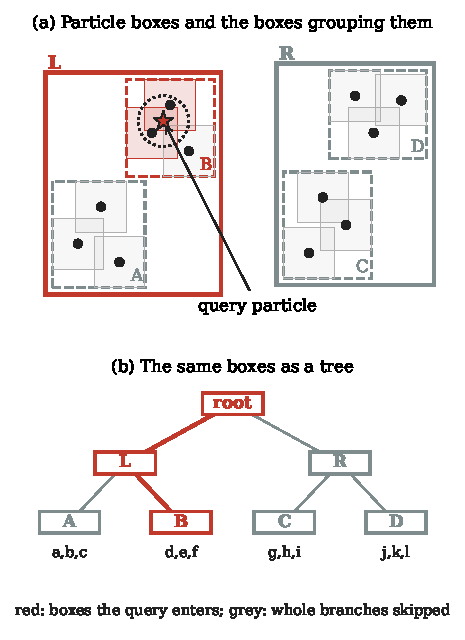
\includegraphics[width=0.95\columnwidth,keepaspectratio]{figures/bvh_diagram.pdf}
\caption{A bounding volume hierarchy over twelve particles. (a) Each particle has a box of half-width $R$; nearby boxes are enclosed in leaf boxes A--D, and those in boxes L and R. (b) The same boxes as a tree. To find the neighbours of the query particle, the search descends only into boxes that contain it (red): branch R is skipped as a whole, and only the particle boxes inside B are tested.}
\label{fig:bvh}
\end{figure}

To find the neighbours of a particle, the search starts at the root and descends only into boxes that contain the query point. Any branch whose box does not contain it is skipped with all the particles below it. At the bottom of the tree only a handful of particle boxes remain, and those are checked with the exact distance test. With a balanced tree a query visits $O(\log N)$ boxes before reaching its candidates.

The BVH has two advantages over the grid. It adapts to the data: dense regions get small boxes and empty regions cost nothing. Each particle's box can also have its own size, so particles with different search radii fit naturally. This is why tree methods dominate astrophysical SPH, where smoothing lengths vary widely. The cost is that the tree must be rebuilt, or at least refitted, every step as the particles move, and that walking a tree involves more irregular memory access and branching than scanning grid cells. Fast parallel builds on the GPU~\cite{karras2012lbvh} make a rebuild every step affordable. The search still has to walk the tree for every particle.

% ======================================================================
\section{Neighbour Search on RT Cores}\label{sec:rt}

Walking a BVH is exactly the work that RT cores do in hardware. In rendering, the question is ``which objects does this ray hit?''. The scene's objects are stored in a BVH, and the RT core walks the tree, testing the ray against each box on the way down, without using the GPU's general-purpose cores~\cite{nvidia2018turing}. We use this hardware through NVIDIA's OptiX library~\cite{parker2010optix}, which runs alongside our CUDA code and reads the same particle arrays in GPU memory.

Neighbour search is not a ray-tracing problem, but it can be rewritten as one~\cite{evangelou2021radius,zhu2022rtnn}. The idea is the one shown in Fig.~\ref{fig:bvh}:
\begin{enumerate}
\item Put a box of half-width $R$ around every particle, and let the hardware build a BVH over these boxes.
\item For each particle $i$, launch one very short ray that starts at $i$'s position. In practice it is little more than a point.
\item A box is ``hit'' when the ray starts inside it, that is, when $i$ lies within distance $R$ of that box's particle along every axis. The hit boxes are exactly the candidate neighbours of $i$, and the RT core finds them by walking the BVH.
\item For each hit, a short piece of our own code, which we call the \emph{per-candidate check}, runs on the normal GPU cores. It computes the true distance, rejects candidates in the corners of the box that lie outside radius $R$, and adds that neighbour's contribution to the density sum~\eqref{eq:density} or the force sum~\eqref{eq:accel}.
\end{enumerate}
One SPH step then proceeds as in Section~\ref{sec:sph}. The BVH is rebuilt from the new positions, one ray per particle computes the densities, pressures follow from~\eqref{eq:eos}, and a second set of rays computes the accelerations. Only the way neighbours are found changes. The kernel, the physics, the integrator and the data layout are the same as in the CUDA grid solver, so the two can be compared directly.

Two properties of this approach shape the comparison. First, RT cores work only in single precision, so the RT solver is single precision and must be compared with a single-precision grid. Second, the hardware speeds up the tree walk, but not the distance test and kernel arithmetic for each candidate, which still run as our own code. That code is invoked once per candidate box the ray reaches. The BVH gives a tighter candidate set than the grid's block of cells. Whether that saving outweighs the cost of invoking our code for every candidate is the question the measurements must answer.

% ======================================================================
\section{GPU Evaluation: From ORCS Benchmarks to SPH Results}\label{sec:gpuresults}

We first compare the CUDA grid with the CPU, because it is the baseline for every RT comparison that follows. We then organized the RT study as a sequence of tests. First, we reproduced ORCS-style spatial distributions to check whether our RT implementation and grid baseline behaved plausibly against published results. We then fixed the comparison conditions and measured complete SPH neighbour sets. Finally, we changed the workload in three ways---adaptive smoothing lengths, Blackwell hardware spheres, and extremely sparse queries---to test whether the fixed-radius result depended on one particular SPH configuration. The last step was to identify the measured cost that explains the results and to determine which published speed-ups depend on different comparison conditions.

\subsection{The CUDA Grid Against the CPU}

We ported the three-dimensional solver and its grid to CUDA, keeping all particle state on the GPU and rebuilding the grid every step with a sort~\cite{green2010cuda}. Table~\ref{tab:gpu} compares it with the 24-thread CPU grid on the same laptop. In single precision the GPU grid is 14 times faster at $10^4$ particles, where fixed launch costs dominate, and 37--40 times faster from $10^6$ particles upward. In double precision it is only about twice as fast as the CPU. This GPU executes 64-bit arithmetic at 1/64 of its 32-bit rate, so at $10^6$ particles the double-precision step takes 18.7 times as long as the single-precision one. The same precision penalty reappears in Section~\ref{sec:why}, where it explains much of the gap between our RT results and published ones.

\begin{table}[!htb]
\centering
\caption{Three-dimensional solver, milliseconds per step on the lattice scene. CPU: 24 threads on the Core Ultra 9 275HX. GPU: RTX 5070 Ti Laptop. Every column uses a grid search.}
\label{tab:gpu}
\footnotesize
\begin{tabular}{@{}rrrrr@{}}
\toprule
 & CPU grid & GPU grid & GPU grid & FP32 vs \\
$N$ & 24 threads & FP64 & FP32 & CPU grid \\
\midrule
$10^4$ & 8.56 & 3.38 & 0.60 & 14$\times$ \\
$10^5$ & 41.7 & 23.3 & 1.37 & 30$\times$ \\
$10^6$ & 343 & 161 & 8.61 & 40$\times$ \\
$10^7$ & 3,109 & 1,428 & 84.8 & 37$\times$ \\
\bottomrule
\end{tabular}
\end{table}

\subsection{Benchmark Protocol}

The study combines full-step and search-only timings. The three-dimensional end-to-end comparison uses a cubic lattice, identical SPH updates, a fixed timestep, two untimed warm-up steps, then 10-step timing windows. The RT solver stores up to 128 neighbours per particle, and no particle exceeded this in the reported runs. Controlled search tests use $N=10^6$ FP32 points and include count, cubic-spline density, and symmetric pressure-plus-viscosity force workloads. The sort-based grid timing includes sorting, cell-range construction, and its query pass. RT time includes building the BVH, or refitting it (resizing the existing boxes to the new positions without rebuilding the tree), plus the search itself. The step that sorts particles into spatial order beforehand is not counted, which favours RT. Each microbenchmark used a one-second warm-up, five repetitions per process, and three independent launches. We report minimum launch time to limit interference from other jobs on the shared Ada workstation. The tests ran on an RTX 5070 Ti Laptop (Blackwell, 46 SMs) and an RTX 5000 Ada (100 SMs), both with OptiX 9.1. Density and force checks had worst relative errors of about $10^{-6}$ and $10^{-5}$; count differences were at most two queries at the FP32 radius boundary.

\subsection{First Test: Reproducing ORCS-Style Distributions}

We began with ORCS's disordered, clustered, and lattice particle sets, with fixed and log-normal search radii. This was a code-quality and comparison-condition check, not yet the SPH result: the published ORCS comparison is a Lennard--Jones workload, so we ran Lennard--Jones forces in the grid and used our RT count-search path. Table~\ref{tab:orcs_control} reports per-SM-normalized times (elapsed milliseconds multiplied by SM count; lower is faster). It places our implementations alongside the corresponding ORCS GPU-CELL and RT-REF results~\cite{meneses2026rtnn}.

\begin{table*}[!htb]
\centering
\caption{ORCS-style distribution check. Per-SM-normalized time (ms $\times$ SM count); values are not direct SPH timings.}
\label{tab:orcs_control}
\scriptsize
\setlength{\tabcolsep}{4.2pt}
\begin{tabular}{@{}l r r r r r@{}}
\toprule
Scenario & ORCS GPU-CELL & Our grid FP32 & Our grid FP64 & Our RT & ORCS RT-REF \\
\midrule
Disordered, $r=1$, $N=10^6$ & 656 & 36.3 & 587 & 139 & 124 \\
Clustered, $r=1$, $N=10^6$ & 1,282 & 41.3 & 750 & 152 & 897 \\
Lattice, $r=1$, $N=10^6$ & 558 & 25.2 & 81 & 111 & 113 \\
Disordered, log-normal, $N=50$k & 24,628 & 473 & 9,169 & 701 & 1,641 \\
Lattice, log-normal, $N=50$k & 24,440 & 473 & 9,152 & 678 & 1,993 \\
Clustered, log-normal, $N=50$k & 43,052 & 474 & 9,915 & 961 & 27,260 \\
\bottomrule
\end{tabular}
\end{table*}

Across these distributions our FP32 grid is 18--91 times faster than our FP64 grid. The FP64 grid, in turn, is within 1.1--1.7 times of ORCS GPU-CELL for fixed-radius cases and 2.7--4.3 times for log-normal cases. This close match is evidence that precision can explain much of the apparent grid penalty, although ORCS does not document GPU-CELL precision, so the FP64 explanation remains an inference. Our RT times are of the same order as ORCS RT-REF on the fixed-radius cases; the RT implementation is therefore not obviously failing because of a grossly inefficient tree build or tree walk. The test also establishes that the clustered, lattice, and disordered cases must be reported separately: their candidate counts and the relative cost of the grid vary substantially.

We next reproduced additional published radius regimes with our own code. On the ORCS log-normal case at 50,000 particles, RT was 1.6--1.8 times slower than a single grid and 10.5--13.6 times slower than the multi-level grid; at 200,000 particles it was about 2.3 times slower than the single grid and 18 times slower than the multi-level grid. We exclude ORCS's uniform-[1,160] results from cross-paper conclusions: their reported throughput is inconsistent with their log-normal case by about an order of magnitude, and the neighbour definition may differ. These replications motivated a fair SPH-specific test rather than treating the published benchmark outcome as the answer for SPH.

\subsection{Second Test: Complete Neighbour Sets for SPH}

For the controlled comparison we used one million points and chose $r=2.754$ to produce about 79 neighbours per query. Both methods used FP32, the same points, GPU-resident data, and complete neighbour sets. Table~\ref{tab:rt_fixed} shows grid / RT times and their ratio. RT loses for count, density, and force on both Blackwell and Ada. In particular, the force test includes the solver's symmetric pressure and Monaghan viscosity terms, so the result is not limited to a count-only proxy.

\begin{table*}[!htb]
\centering
\caption{Complete FP32 SPH search timings at $N=10^6$, $k\approx79$. Each cell is grid / RT time (ms) and RT divided by grid.}
\label{tab:rt_fixed}
\scriptsize
\begin{tabular}{@{}l r r@{}}
\toprule
Workload & RTX 5070 Ti Laptop (Blackwell) & RTX 5000 Ada \\
\midrule
Neighbour count & 3.26 / 11.85 (3.64$\times$) & 1.71 / 6.17 (3.60$\times$) \\
SPH density & 3.38 / 12.74 (3.77$\times$) & 1.87 / 6.70 (3.58$\times$) \\
Pressure and viscosity force & 5.68 / 17.63 (3.11$\times$) & 3.08 / 9.06 (2.94$\times$) \\
\bottomrule
\end{tabular}
\end{table*}

Fig.~\ref{fig:ksweep} repeats the count test from 1 to 512 neighbours per particle. With the BVH rebuilt for every search, RT is 3.2--5.2 times slower at every neighbour count on both GPUs. Refitting the existing BVH instead of rebuilding it helps most when there are few neighbours, but it reaches parity with the grid only near one neighbour per particle (1.02 and 1.16 times). Only the search on its own, with all BVH cost removed, beats the grid, and only below about three neighbours. SPH, at 50--100 neighbours, is far from that regime.

\begin{figure*}[!htb]
\centering
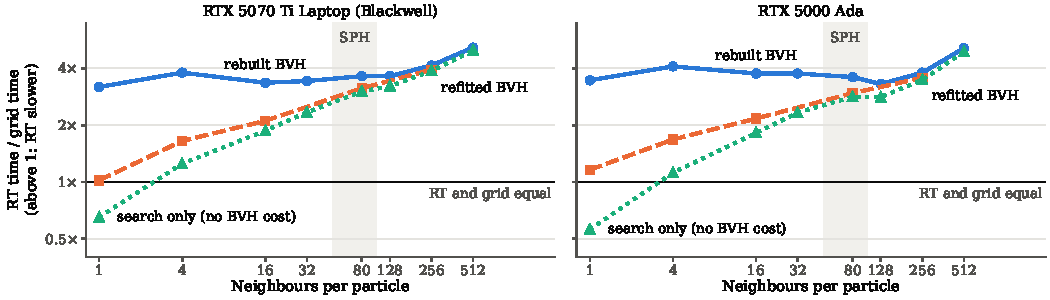
\includegraphics[width=\textwidth,keepaspectratio]{figures/rt_ksweep.pdf}
\caption{RT time divided by grid time against neighbours per particle ($N=10^6$, count workload, minimum of three launches). Above the black line RT is slower. The shaded band marks SPH neighbour counts. ``Search only'' excludes all BVH construction and refit cost, so it is a lower bound for RT.}
\label{fig:ksweep}
\end{figure*}

The full-step result points the same way. At one million particles the CUDA grid takes 8.53~ms per step and the OptiX solver 17.29~ms; at four million the times are 33.60 and 68.52~ms. The end-to-end gap is about 2.0 times, smaller than the isolated-search gap because integration and other work are common to both. The RT list capacity remained 128 with no overflow in these runs.

\subsection{Three Follow-Up Cases}

\textbf{Adaptive smoothing lengths.} We compared RT against a multi-level grid, assigning particles to bounded grids by powers-of-two radius levels. On Ada, this grid was 1.35--1.98 times faster across the tested adaptive profiles and two-level scenes at $N=10^6$. In the stress test, increasing the radius range from 100 to nearly 10,000 while holding the average near 81 neighbours kept multi-level-grid time between 4.93 and 5.39~ms, while RT increased from 7.28 to 9.12~ms. Thus the grid's advantage widened from 1.35 to 1.84 times. A previous proof-of-concept comparison had used only a single grid sized to the largest radius; it produced large apparent RT wins, but those did not survive the multi-level baseline. Fig.~\ref{fig:multires}(a) shows why: that single grid slows by three orders of magnitude as the ratio between coarse and fine $h$ grows, while RT and the multi-level grid both stay flat, with the grid faster.

\begin{figure}[!htb]
\centering
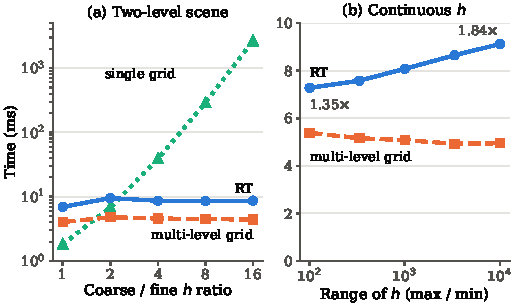
\includegraphics[width=\columnwidth,keepaspectratio]{figures/rt_multires.pdf}
\caption{Adaptive smoothing lengths on the RTX 5000 Ada ($N=10^6$, about 80 neighbours per particle). (a) Two-level scene: a single grid sized for the coarse radius grows by three orders of magnitude, while RT and the multi-level grid stay flat. (b) Continuous $h$ following the particle density: the multi-level grid stays flat as the range widens and RT slows, so its deficit grows from 1.35 to 1.84 times.}
\label{fig:multires}
\end{figure}

\textbf{Blackwell hardware spheres.} The newest GPUs can test a ray against a sphere directly in hardware, which could replace our software distance check. We found, however, that a hardware sphere reports no hit when the ray starts inside it, so it cannot directly answer ``is this point inside the sphere?''. The only correct alternative was a longer ray that ends at the query point, and a longer ray reaches more boxes. With rays of the same length, the hardware spheres cut the number of candidates our code had to examine by about three times, but the search was still 16\% slower than with plain boxes. Overall this path was 7--10 times slower than the grid, so the hardware feature does not change the SPH result.

\textbf{Ultra-sparse queries.} We tested one million points in a mostly empty domain with about one neighbour per query. A rebuilt BVH was 1.4--4.3 times slower than a compact grid. Replacing rebuild with refit gives an estimated 1.5--2.5 times RT advantage, based on the measured search and refit times; this is a narrow regime-specific estimate, not a measured end-to-end win. It identifies a plausible RT niche, but it is far from the tens of neighbours per particle in the SPH tests.

\subsection{Why the SPH Result Persists}\label{sec:why}

The follow-up tests point to a cost floor in the RT search path, rather than a single poor setting. Table~\ref{tab:ablate} lists the variants we tried, and none brings RT below the grid. Refitting the BVH instead of rebuilding it still leaves RT 3.0--3.1 times slower. A BVH tuned for faster search removes about 10\% of the candidates but costs more to build. Excluding the BVH entirely still leaves the search alone 2.8--3.0 times slower. Putting the queries in random order makes RT 45--78\% slower, which confirms that our spatially sorted queries already apply the main optimisation reported for RTNN~\cite{zhu2022rtnn}.

\begin{table}[!htb]
\centering
\caption{RT variants at $N=10^6$ and about 79 neighbours per particle (count workload). Each value is RT time divided by grid time; above 1 means RT is slower.}
\label{tab:ablate}
\footnotesize
\begin{tabular}{@{}lrr@{}}
\toprule
RT variant & Laptop & Ada \\
\midrule
Standard search, BVH rebuilt every call & 3.64 & 3.60 \\
BVH refitted instead of rebuilt & 3.14 & 2.96 \\
BVH built for faster search & 3.56 & 3.55 \\
Search only, BVH cost excluded & 3.02 & 2.83 \\
Per-candidate check doing no work$^{a}$ & 2.08 & 1.91 \\
Hits passed to a second routine (our solver) & 4.42 & 4.27 \\
Queries in random order & 5.27 & 6.40 \\
Hardware sphere primitive & 7.95 & 10.27 \\
\midrule
\multicolumn{3}{@{}l}{Work per query: 78.6 neighbours. RT checks 180.8 candidates} \\
\multicolumn{3}{@{}l}{(2.30 per neighbour); the grid tests 505.7 (6.43 per neighbour).} \\
\bottomrule
\end{tabular}

\vspace{2pt}
{\scriptsize $^{a}$Search time only; the check returns no result, so this is a lower bound.}
\end{table}

At $k\approx79$, RT ran the per-candidate check 181 times per particle (2.30 times per true neighbour), whereas the grid performed 506 distance tests (6.43 per neighbour). Each run of the check cost about eight times a grid distance test on both GPUs. Even a check that did no work at all cost about 5.5 times as much, so most of the cost lies in reaching and starting the check for each candidate, not in the arithmetic inside it. A fitted cost model predicted the winner correctly at all 18 held-out neighbour-count points. If an ideal BVH produced only one candidate per true neighbour, our measured costs extrapolate to roughly parity with the grid, and adding the measured refit cost leaves it near parity. These ideal-BVH figures are estimates, but they show that the BVH's smaller candidate set is not enough to pay for the per-candidate cost at SPH neighbour counts.

Our solver currently passes each accepted neighbour to a second routine before adding its contribution. That path is 23--32\% slower than adding the contribution directly inside the check, so implementation choices do matter. Fixing it cannot close the 3--4 times gap, however. The decisive property of the workload is that SPH needs the contribution of every one of many neighbours. On the RT path every candidate costs a run of our own code, while the grid tests candidates with a few cheap arithmetic operations in a simple loop. This is an interaction between the SPH density and force workload and the way RT hardware is programmed, not evidence that our RT implementation is simply unoptimised. It does not establish that all RT hardware or all SPH regimes must lose.

We then added suspected literature confounds one at a time to the same input (Fig.~\ref{fig:confounds}). On the laptop, the fair comparison at $k\approx79$ gave grid / RT = 3.20 / 11.92~ms, so the grid was 3.7 times faster. Changing only the grid to FP64 made it 12.9 times slower (12.3 on Ada) and turned the result around: RT appeared 3.5 times faster (3.3 on Ada). Adding a re-upload of the positions and a copy of the full neighbour lists to the host on the grid side, as a library that returns its results to the CPU does, raised the apparent RT advantage to 6.5 times (7.7 on Ada). Stopping the RT search after 50 neighbours, as RTNN's range search does by default, returned only 63\% of the true neighbours and raised the laptop figure further to 7.9 times.

\begin{figure}[!htb]
\centering
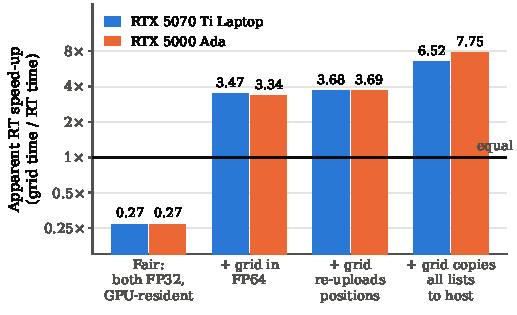
\includegraphics[width=\columnwidth,keepaspectratio]{figures/rt_confounds.pdf}
\caption{Adding comparison conditions found in published baselines to a fair test ($N=10^6$, about 79 neighbours, the same points for both methods, RT search complete). Values above 1 mean RT appears faster. Making only the grid double precision reverses the result on both GPUs.}
\label{fig:confounds}
\end{figure}

Reading the public source code shows that these conditions exist in practice. RTNN's range search stops at 50 neighbours by default~\cite{zhu2022rtnn}. cuNSearch, the grid library RTNN compares against, defaults to double precision and copies its full neighbour lists to the host on every search. We did not run either program ourselves, and the exact configuration used in the RTNN paper is not verified. ORCS GPU-CELL precision is also unreported, so its match to our FP64 grid remains an inference~\cite{meneses2026rtnn}. The bridge tests demonstrate how these choices can reverse a result; they do not prove that every published speed-up used all of them.

\subsection{Scope of the Evidence}

The experiments use NVIDIA GPUs and OptiX 9.1 only. The Ada workstation was shared; minimum-over-launch reporting reduces but cannot remove contention. Refit was measured with frozen particles, which favours RT, and RT totals exclude Morton reordering. The multi-level-grid build includes a small device-to-host copy and is not fully optimized. Direct head-to-head builds of RTNN and cuNSearch were not completed; AMD hardware, other ray-tracing libraries, and energy use were not tested. The variable-radius tests use a scatter rule, not the symmetric maximum-radius rule. Finally, the sequential physical validation is two-dimensional, while these GPU tests establish search correctness and performance rather than experimental accuracy or trajectory-level agreement of all solvers.

% ======================================================================
\section{Conclusion}\label{sec:conclusion}

Neighbourhood search is the dominant cost in the sequential SPH solver: it accounts for 93.6\% of the measured step at 2,030 particles and 99.3\% at 30,016. OpenMP distributes the all-pairs work effectively across CPU cores, reaching a 15.4$\times$ speed-up at 99,960 particles, but retains quadratic candidate search. Replacing all-pairs search with a uniform grid changes the work performed and produces the largest measured CPU improvement: at 99,960 particles, the 24-thread grid is about 229 times faster than the 24-thread all-pairs implementation.

On the GPU, the CUDA grid also outperformed the tested RT-core solver in end-to-end measurements. At one million particles the grid completed a step in 8.53~ms, versus 17.29~ms for RT. Controlled experiments on Blackwell and Ada GPUs show a larger gap for the search itself: with complete FP32 neighbour sets at SPH-like counts, RT takes about three to four times the grid time for count, density, and force workloads. Counting the work shows why. Each candidate the RT hardware finds costs a run of our own check code, about eight times as expensive as a grid distance test, and this outweighs the BVH's smaller candidate set. For adaptive smoothing lengths, a multi-level grid remains faster and the gap grows as the radius range widens.

The evidence supports keeping grid-based neighbourhood search in this solver. RT cores may suit very sparse query workloads, but the tested RT implementation does not accelerate the measured SPH regimes. Cross-paper comparisons should report precision, neighbour completeness, data-transfer boundaries, and the grid representation because each can materially affect the result.

These conclusions concern performance and the tested implementations. The physical validation remains incomplete: the dam-break comparison to experimental front data is not yet quantitative, the hydrostatic pressure gradient and free-surface height remain discrepant, and GPU solver states have not been compared over matched trajectories. Resolving those validation issues, recording full compiler and hardware metadata, and completing direct third-party implementations would strengthen a future evaluation.

% ======================================================================
\bibliographystyle{IEEEtran}
\bibliography{references}

\end{document}
